\newpage

\begin{figure}[htbp]
    \centering
    \makebox[\textwidth][c]{%
        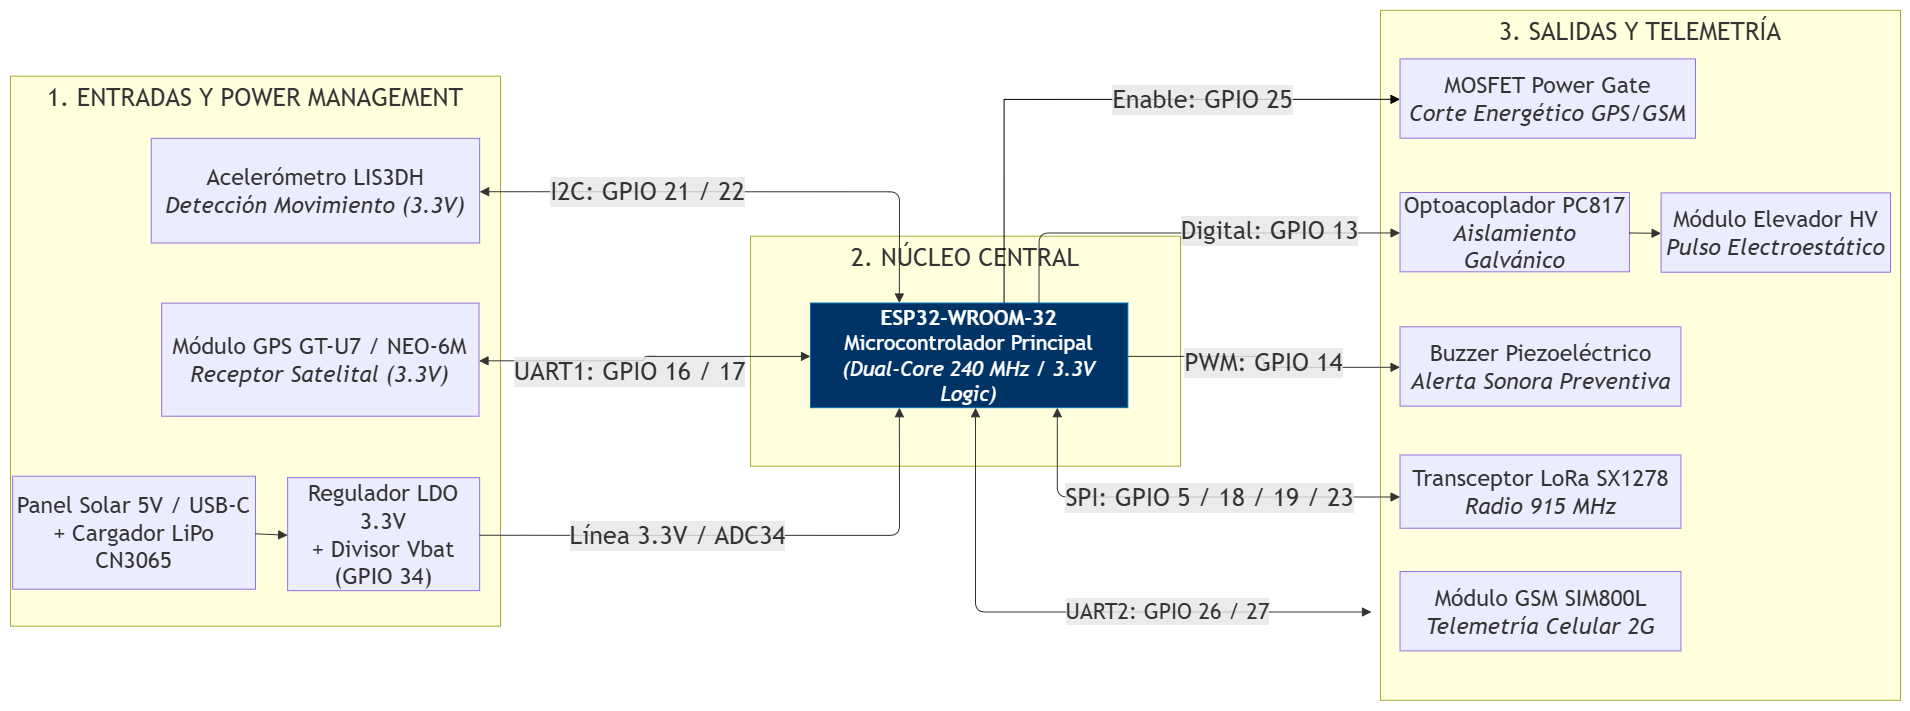
\includegraphics[width=1.1\textwidth]{Secciones/Figuras/diagrama_bloques_hardware.png}%
    }
    \vspace{0.3cm}
    \caption{Diagrama de bloques de la arquitectura de hardware del sistema DR-VF-01.}
    \label{fig:diagrama_hardware}
\end{figure}

\clearpage
%Tabla de mapeo de pines
\section*{Mapeo de Pines y Asignación de Periféricos}

\begin{table}[H]
    \centering
    \small
    \renewcommand{\arraystretch}{1.3}
    \rowcolors{2}{white}{gray!8}
    \begin{tabularx}{\linewidth}{|c|c|c|X|}
        \hline
        \rowcolor{gray!20}
        \textbf{Módulo / Periférico} & \textbf{Protocolo / Función} & \textbf{Pines ESP32} & \textbf{Notas para el Esquemático / PCB} \\ \hline
        GPS (GT-U7) & UART1 & GPIO 16 (RX), GPIO 17 (TX) & Intercambiar TX/RX en el ruteo de la PCB. \\ \hline
        GSM (SIM800L) & UART2 & GPIO 26 (RX), GPIO 27 (TX) & Requiere pista ancha de alimentación (picos de $2~\text{A}$). \\ \hline
        IMU (LIS3DH) & $\text{I}^2\text{C}$ & GPIO 21 (SDA), GPIO 22 (SCL) & Agregar resistencias pull-up de $4.7~\text{k}\Omega$ en la PCB. \\ \hline
        LoRa (SX1278) & SPI & GPIO 5 (CS), 18 (SCK), 19 (MISO), 23 (MOSI) & Mapear señal GPIO 4 para interrupción. \\ \hline
        Buzzer Piezoeléctrico & PWM & GPIO 12 & Control mediante transistor NPN o MOSFET. \\ \hline
        Optoacoplador PC817 & Digital Output & GPIO 13 & Mantener separación de planos de masa (\texttt{GND} vs. \texttt{HV\_GND}). \\ \hline
        MOSFET Power Gate & Power Control & GPIO 25 & Transistor P-Channel / N-Channel según topología. \\ \hline
        Monitoreo Batería & ADC1 & GPIO 34 & Solo entrada (\textit{Input Only}), ideal para divisor resistivo. \\ \hline
    \end{tabularx}
\end{table}


%Arbol de Potencia
\clearpage
\begin{figure}[htbp]
    \centering
    \resizebox{\linewidth}{!}{%
    \begin{tikzpicture}[
        pwr/.style={rectangle, draw=orange!80!black, fill=orange!10, thick, text width=2.4cm, text centered, rounded corners=3pt, minimum height=1.1cm, font=\sffamily\small},
        bus/.style={rectangle, draw=blue!80!black, fill=blue!10, thick, text width=2.4cm, text centered, rounded corners=3pt, minimum height=1.1cm, font=\sffamily\small},
        gate/.style={rectangle, draw=red!80!black, fill=red!10, thick, text width=2.4cm, text centered, rounded corners=3pt, minimum height=1.1cm, font=\sffamily\small},
        load/.style={rectangle, draw=gray!80, fill=gray!10, text width=2.2cm, text centered, rounded corners=3pt, minimum height=1.0cm, font=\sffamily\footnotesize},
        arrow/.style={draw, -{Latex[scale=0.9]}, thick, color=gray!70!black}
    ]

        % Capa 0: Fuentes de Entrada y Almacenamiento (y = 0)
        \node [pwr] (in) at (0,0) {Entrada 5V\\(Solar / USB-C)};
        \node [pwr] (charger) at (3.6,0) {Cargador LiPo\\(CN3065)};
        \node [pwr] (bat) at (7.2,0) {Batería LiPo\\(3.7V -- 4.2V)};

        \draw [arrow] (in) -- (charger);
        \draw [arrow] (charger) -- (bat);

        % Capa 1: Gestión y Regulación Principal (y = -2.6)
        \node [load] (gsm) at (0,-2.6) {Módulo GSM\\SIM800L\\(Picos $\le 2\text{A}$)};
        \node [bus] (ldo) at (3.6,-2.6) {Regulador LDO\\3.3V (ME6211)};
        \node [gate] (mosfet) at (7.2,-2.6) {MOSFET\\Power Gate\\(GPIO 25)};

        % Riel principal VBAT (y = -1.3)
        \draw [thick, color=gray!70!black] (bat.south) -- (7.2,-1.3);
        \node[right=3pt, font=\tiny\bfseries, color=orange!90!black] at (7.2,-0.9) {$V_{\text{BAT}}$};

        \draw [thick, color=gray!70!black] (7.2,-1.3) -- (0,-1.3);
        \draw [arrow] (0,-1.3) -- (gsm.north);
        \draw [arrow] (3.6,-1.3) -- (ldo.north);
        \draw [arrow] (7.2,-1.3) -- (mosfet.north);
        
        \node[above=2pt, font=\tiny\bfseries, color=orange!90!black] at (1.8,-1.3) {$V_{\text{BAT}}$};
        \node[above=2pt, font=\tiny\bfseries, color=orange!90!black] at (5.4,-1.3) {$V_{\text{BAT}}$};

        % Capa 2: Consumidores y Periféricos (y = -5.4)
        \node [load] (sensors) at (0,-5.4) {Sensores / Radio\\(LIS3DH / SX1278)};
        \node [load] (esp) at (2.8,-5.4) {ESP32-WROOM\\(Microcontrolador)};
        \node [load] (hv) at (5.6,-5.4) {Elevador HV\\(Pulso Eléctrico)};
        \node [load] (gps) at (8.4,-5.4) {Módulo GPS\\GT-U7};

        % Riel 3.3V (Salida LDO a y = -4.0)
        \draw [thick, color=gray!70!black] (ldo.south) -- (3.6,-4.0);
        \node[right=4pt, font=\tiny\bfseries, color=blue!80!black] at (3.6,-3.5) {3.3V};
        
        \draw [thick, color=gray!70!black] (3.6,-4.0) -- (0,-4.0);
        \draw [thick, color=gray!70!black] (3.6,-4.0) -- (2.8,-4.0);
        \draw [arrow] (0,-4.0) -- (sensors.north);
        \draw [arrow] (2.8,-4.0) -- (esp.north);

        % Riel V_SW Conmutado (Salida MOSFET a y = -4.0)
        \draw [thick, color=gray!70!black] (mosfet.south) -- (7.2,-4.0);
        \node[right=4pt, font=\tiny\bfseries, color=red!80!black] at (7.2,-3.5) {$V_{\text{SW}}$};

        \draw [thick, color=gray!70!black] (7.2,-4.0) -- (5.6,-4.0);
        \draw [thick, color=gray!70!black] (7.2,-4.0) -- (8.4,-4.0);
        \draw [arrow] (5.6,-4.0) -- (hv.north);
        \draw [arrow] (8.4,-4.0) -- (gps.north);

    \end{tikzpicture}%
    }
    \caption{Árbol de distribución de potencia y gestión energética para el sistema DR-VF-01.}
    \label{fig:arbol_potencia}
\end{figure}

%Tabla de Presupuesto Energético (Power Budget).
\section*{Presupuesto Energético y Perfil de Consumo}

\begin{table}[H]
    \centering
    \small
    \renewcommand{\arraystretch}{1.3}
    \rowcolors{2}{white}{gray!8}
    \begin{tabularx}{\linewidth}{|X|c|c|c|c|}
        \hline
        \rowcolor{gray!20}
        \textbf{Subcircuito / Módulo} & \textbf{Riel Alimentación} & \textbf{Consumo Activo} & \textbf{Consumo Reposo} & \textbf{Estado MOSFET} \\ \hline
        ESP32-WROOM & LDO $3.3~\text{V}$ & $160~\text{mA}$ & $10~\mu\text{A}$ (\textit{Deep Sleep}) & Siempre ON \\ \hline
        Sensores (LIS3DH / SX1278) & LDO $3.3~\text{V}$ & $12~\text{mA}$ & $2~\mu\text{A}$ & Siempre ON \\ \hline
        Módulo GSM (SIM800L) & Directo $V_{\text{BAT}}$ & $350~\text{mA}$ (Picos $2~\text{A}$) & $1~\text{mA}$ (\textit{Standby}) & Siempre ON \\ \hline
        Módulo GPS (GT-U7) & Conmutado $V_{\text{SW}}$ & $45~\text{mA}$ & $0~\text{mA}$ (Desconectado) & OFF en Reposo \\ \hline
        Elevador HV (Pulso) & Conmutado $V_{\text{SW}}$ & $80~\text{mA}$ (Puntual) & $0~\text{mA}$ (Desconectado) & OFF en Reposo \\ \hline
        \textbf{Consumo Total Promedio} & -- & \textbf{$\approx 647$ mA} & \textbf{$\approx 1.01$ mA} & -- \\ \hline
    \end{tabularx}
\end{table}